\chapter{Introduction}

\lettrine[findent=.1em,lines=2,nindent=0em]{S}{oftware} and hardware systems are becoming more and more complex. At the same time, such systems are increasingly used by nonexperts\,---\,albeit consciously or unconsciously. With the growing influence of computerized systems on nearly every aspect of today's life, \emph{correctness} is of paramount importance in such ubiquitous environments. Incorrect systems, which expose bugs and undefined or unpredictable behavior, do not just affect technical systems any more, but may threaten life in safety-critical systems or compromise the reputation or economical situation of individuals, companies, or governments. A cost analysis from 2002~\cite{nist_2002} estimates software bugs to cost alone the \acronym{U.S.}~economy nearly 60 billion \acronym{U.S.}~dollars a year. This number is growing as a survey from 2008~\cite{idc_2008} already reports annual debugging costs for single North American companies of up to 22 million \acronym{U.S.}~dollars.

Although postulated for several decades, especially \emph{software systems are not yet designed and implemented in an engineering fashion}. Hence, complex systems usually contain design flaws. This may be because of faster production cycles, benefit-cost analyses, or the sheer size of systems. To still ensure correctness, different approaches have been proposed in the previous decades. From a conceptual point of view, domain-specific languages have been introduced to ease the complexity of specifying systems. They aim at abstracting from specifics (\eg, assembly language or gate-level descriptions) and allow to specify the desired behavior at a human-understandable level of detail, for instance using high-level programming languages such as Java or \acronym{VHDL}. Such languages allow for an intuitive and brief implementation of a system and can help to prevent design flaws in the first place.

As the choice of language does not guarantee correctness alone, bugs often need to be detected in already running systems. As it is undesirable to discover these bugs when the system is operational, \emph{extensive testing is needed}. Testing is an empirical method observing the system's output on given inputs and comparing this output to expected results. This technique is especially effective for software systems or any other system whose behavior can be simulated. The flexibility and nonmaterial nature of software further allows to fix already running systems once a design flaw is detected. Whereas this approach is reasonably cheap and fairly acceptable in noncritical environments, it does not guarantee correctness but just the absence of concrete design flaws in the test runs of the system\,---\,testing inherently can only detect the presence of bugs, but not their absence. Notwithstanding, the integration of testing into the development process (called test-driven development) can detect and fix many design flaws in an early stage which in turn may dramatically reduce overall development costs~\cite{Moody_2005_dke}.

The only way to guarantee the correctness of a system is to use \emph{formal methods}. Instead of investigating a given concrete system or its outputs, it is translated into a mathematical model on which correctness can be proven. Of course, the model must cover all important aspects of the concrete system that are relevant for the property that needs to be verified. If the model abstracts from important details, it may be proved correct, whereas the implementation still contains errors. For these reasons, formal methods are, compared with testing, expensive and time-consuming, but the only possibility to verify every aspect of life-critical or economically vital systems. However, a formal correctness proof has the disadvantage to be complex and hard to automate. Even worse, proofs tend not to scale with the size of the system under consideration.

To automate verification without losing rigor, \emph{model checking}~\cite{ClarkeGD_1999_book} has been introduced. Model checking treats the verification problem as a search problem in which undesired states (\ie,~bugs) are searched in a graph which models the system's behavior. Even though this state graph usually underlies exponential growth in case the number of components is increased, modern techniques allow for model checking of large industrial systems such as hardware circuits, communication protocols, or software drivers. These techniques include abstraction (\ie,~irrelevant properties of the system are not modeled or verified), compact representation (\eg, a symbolic representation of the state graph using binary decision diagrams~\cite{Bryant_1986_tc}), and compositionally (\ie,~deducing the system's correctness from the correctness of its components). Nevertheless, these techniques do not yet scale to large software programs such as operating systems and enterprise systems.

Nowadays, the usage of model checking tools and the formalization of systems and properties are much easier than conducting formal proofs. Additionally, model checking techniques usually return a counterexample which points out a situation in which the model does not meet a specification. A counterexample can help the modeler understand and locate a flaw in the original system where it can be fixed. By iterating model checking and error removal, correctness can be eventually proved\,---\,assuming the system is realizable. The approach to achieve correctness this way is called \emph{correctness by verification}.

A different approach to achieve correctness is \emph{correctness by construction}. In this realm, a system or model is constructed from a specification and the correctness immediately follows from the correctness of the construction algorithm. Such completion, recommendation, or correction algorithms focus on the design phase of a system and aim at avoiding design flaws as early as possible. To this end, correctness by construction combines the rigor of verification and the simplicity of test-driven development. However, such constructed models usually need to be refined manually toward actual implementations.

To conclude, different approaches exist to ensure the correctness of systems. They differ in the degrees of maturity and applicability to real-life systems. A close integration of verification techniques into the design process enables the cost-efficient development of correct systems and is a step toward engineering of systems.

\bigskip

%%%%%%%%%%%%%%%%%%%%%%%%%%%%%%%%%%%%%%%%%%%%%%%%%%%%%%%%%%%%%%%%%%%%%%%%%%%%%%
\begin{figure}
\centering
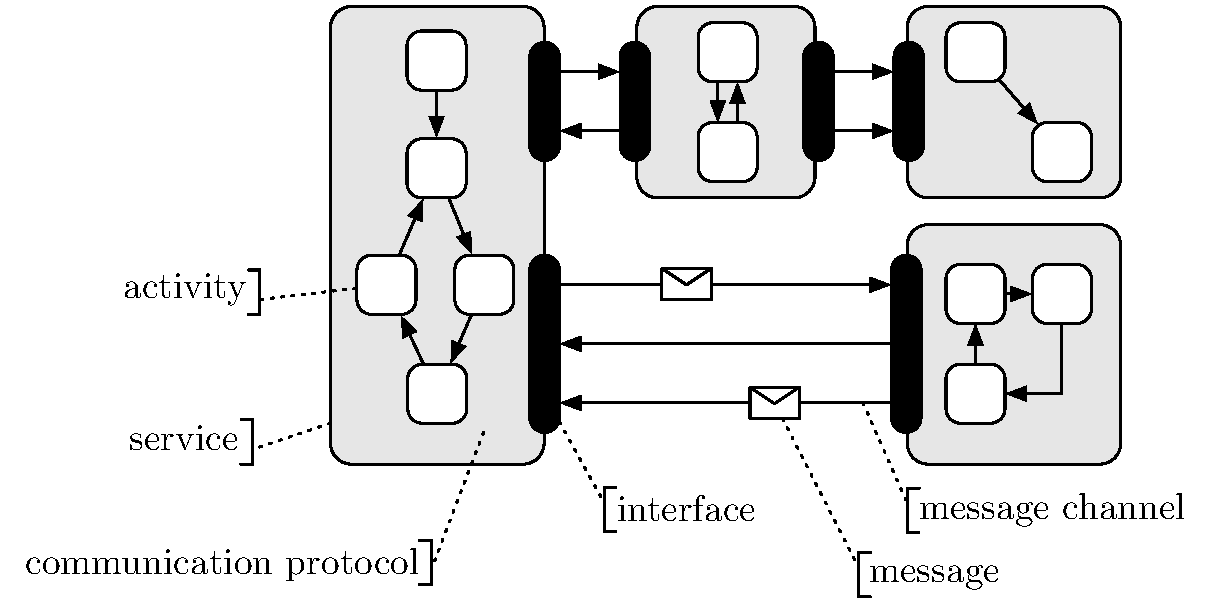
\includegraphics[scale=0.4]{introduction/overview}\hspace{4em}
\caption{A service composition.}
\label{fig:overview}
\end{figure}
%%%%%%%%%%%%%%%%%%%%%%%%%%%%%%%%%%%%%%%%%%%%%%%%%%%%%%%%%%%%%%%%%%%%%%%%%%%%%%

\noindent\emph{Service-oriented computing} (\acronym{SOC})~\cite{Papazoglou_2001_cacm} is an emerging paradigm of interorganizational cooperation. It aims at breaking complex monolithic systems into a composition of several simpler and self-contained, yet logically or geographically distributed components, called \emph{services}. A service has an identifier and offers an encapsulated functionality through a well-defined interface; see \autoref{fig:overview} for an illustration of the concepts. Services are open systems and are designed for being invoked by other services or for invoking other services themselves, and are typically not executed in isolation. Conceptually, \acronym{SOC} revives old ideas from component-based design~\cite{Mcilroy_1969_sect,Szyperski_1998_book} or from programming-in-the-large~\cite{DeRemerK_1976_tse}, for instance.

A simple realization of \acronym{SOC} is the encapsulation of classical computer programs which calculate an output from given inputs as \emph{remote procedure calls} or \emph{stateless services}. Such services only exchange pairs of request/response messages and are capable of implementing simple systems such as stock or weather information systems. This approach is insufficient to implement real-world business scenarios, which do not only calculate an output from given inputs, but in which messages are constantly sent back and forth. Examples for such \emph{stateful} conversations are price negotiations, auctioning, or scenarios in which exception handling is necessary. In this setting, more complex interactions need to be considered and a service needs to implement a \emph{communication protocol} (also called \emph{business protocol}~\cite{Papazoglou_2007_book}) which specifies the order in which the service's activities are executed and which may distinguish arbitrary states of the interaction with other services. The most prominent class of services are \emph{Web services}~\cite{AlonsoCKM_2003}. Here, the Internet and several Web-related standards are used to realize \acronym{SOC}. This makes services virtually independent of their geographical location and technological context and allows to entirely focus on the functions a service offers.

%%%%%%%%%%%%%%%%%%%%%%%%%%%%%%%%%%%%%%%%%%%%%%%%%%%%%%%%%%%%%%%%%%%%%%%%%%%%%%
\begin{figure}
\centering
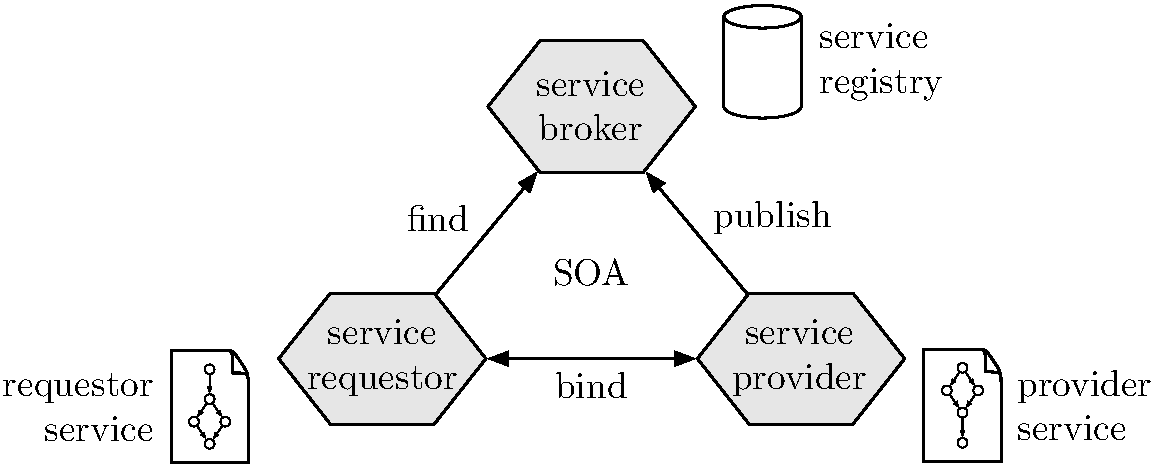
\includegraphics[scale=0.4]{introduction/soa-triangle}
\caption{The \acronym{SOA} triangle.}
\label{fig:soatriangle}
\end{figure}
%%%%%%%%%%%%%%%%%%%%%%%%%%%%%%%%%%%%%%%%%%%%%%%%%%%%%%%%%%%%%%%%%%%%%%%%%%%%%%

The idea of abstracting from underlying technologies and implementations makes it possible to compare services and to replace one service by another service which is, for instance faster, cheaper, compliant with new legal regulations, or more reliable. To this end, \acronym{SOC} allows to effortlessly replace, outsource, and optimize functionalities. This flexible binding is described as a \emph{service-oriented architecture} (\acronym{SOA})~\cite{Gottschalk00}. A \acronym{SOA} provides a general framework for service interaction. This framework\,---\,often called the \acronym{SOA} triangle\,---\,distinguishes three roles of services (as shown in \autoref{fig:soatriangle}). A \emph{service provider} publishes information about his service to a public registry. A \emph{service broker} manages the registry and allows a \emph{service requester} to find an adequate published service. Then, the provider and the requester may bind their services and start interaction.

%%%%%%%%%%%%%%%%%%%%%%%%%%%%%%%%%%%%%%%%%%%%%%%%%%%%%%%%%%%%%%%%%%%%%%%%%%%%%%
\begin{figure}
\centering
\hfill
\subfigure[service orchestration\label{fig:intro:orch}]{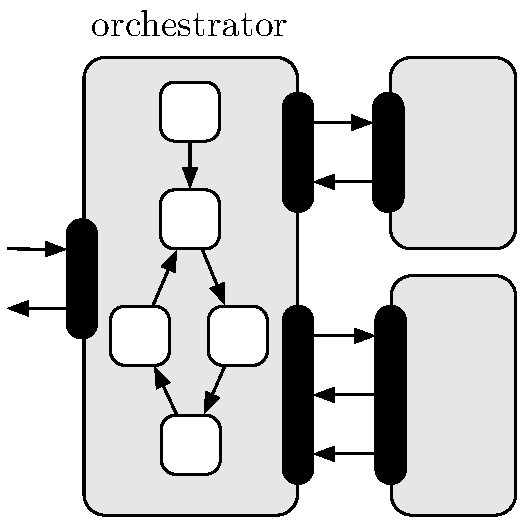
\includegraphics[scale=0.4]{introduction/orchestrator}}\hfill
\subfigure[service choreography\label{fig:intro:chor}]{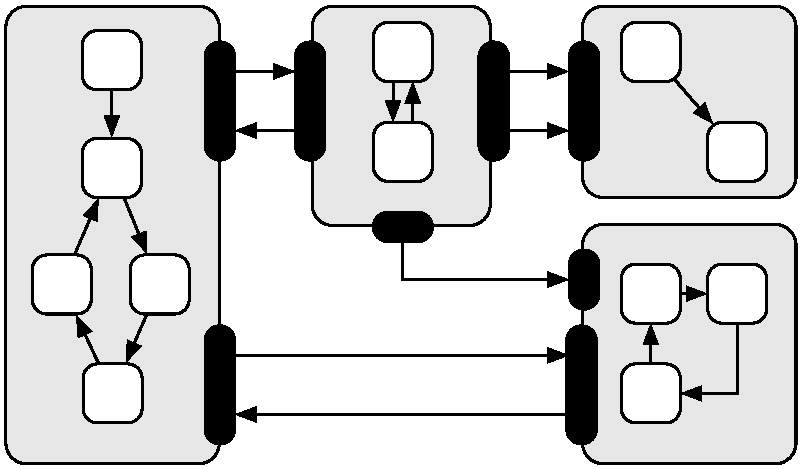
\includegraphics[scale=0.4]{introduction/choreography}} \hfill${}$
\caption{Service orchestration versus service choreography.}
\end{figure}
%%%%%%%%%%%%%%%%%%%%%%%%%%%%%%%%%%%%%%%%%%%%%%%%%%%%%%%%%%%%%%%%%%%%%%%%%%%%%%

In a \emph{service orchestration}, the flexibility to bind formerly unknown providers is employed to offer higher-value added services. It takes the viewpoint of a single participant in the service composition (the \emph{orchestrator}) and abstracts from the internal behavior of other participants. The orchestrator only considers the interfaces of the other participants rather than their concrete behavior or any interaction between third parties (see \autoref{fig:intro:orch}). Service orchestrations are well-suited to describe a business process whose activities are executed by other services.

Services can be also used to specify and implement an entire interorganizational business process. Such a business process is specified by several parties and explicitly or implicitly describes the behavior of each participant from a global perspective (see~\autoref{fig:intro:chor}). From this public description (also called \emph{contract} or \emph{service choreography}), each party derives its share and implements it as a service.

Services received much attention in industry and academia. This is reflected by many standardization efforts for several aspects of services. For instance, there exist various specification and programming languages for services orchestrations (\eg, \acronym{WS-BPEL}~\cite{standard_bpel} or \acronym{BPMN}~\cite{standard_bpmn}) and choreographies (\eg, \bpelchor~\cite{DeckerKLW_2007_icws}, \acronym{WS-CDL}~\cite{standard_wsdl}, i\acronym{BPMN}~\cite{DeckerB_2007_bpmw}, or \acronym{BPMN} 2.0 choreographies~\cite{standard_bpmn2}).





%%%%%%%%%%%%%%%%%%%%%%%%%%%%%%%%%%%%%%%%%%%%%%%%%%%%%%%%%%%%%%%%%%%%%%%%%%%%%%%
\section{Research goal}
%%%%%%%%%%%%%%%%%%%%%%%%%%%%%%%%%%%%%%%%%%%%%%%%%%%%%%%%%%%%%%%%%%%%%%%%%%%%%%%

Service-orientation allows to construct large distributed systems by composing several heterogenous and decentralized services. This modularization may reduce complexity and cost. At the same time, new challenges arise with the distributed execution of independent services in flexible compositions. In particular, the correctness of a service composition depends on the local correctness of each participating service \emph{and} the correct interaction between them. Unlike in a centralized monolithic system, parts of the system may change and are not completely controlled by a single party. Furthermore, a global state of the system and transitions between states are replaced by local states and local state transitions in addition to message transfer between parties.

Although services have been around for many years and several scientific communities focus on service-related topics, there do not exist widely accepted correctness criteria which are specific to services. From a practical point of view, a system composed of several services can be considered correct if it behaves just as well as a monolithic system. In particular, \emph{the participants should not be aware that the system consists of several decentrally executed components which implement a complex communication protocol and that have been bound without revealing specific implementation details}.

This brings us to the central research question which is investigated in this thesis:

%%%%%%%%%%%%%%%%%%%%%%%%%%%%%%%%%%%%%%%%%%%%%%%%%%%%%%%%%%%%%%%%%%%%%%%%%%%%%%
\begin{framed}
\noindent How can the design of correct services and service compositions be systematically supported?
\end{framed}
%%%%%%%%%%%%%%%%%%%%%%%%%%%%%%%%%%%%%%%%%%%%%%%%%%%%%%%%%%%%%%%%%%%%%%%%%%%%%%

This question touches upon several challenges:
\begin{niceitemize}
\item \emph{Formalization and verification of correctness.} How to formalize service behavior and correctness notions for services? Can correctness be automatically verified using model checking techniques?
\item \emph{Error detection and correction.} In case an error is detected, which participating services are responsible for this error? How can the overall system be fixed toward correct execution?
\item \emph{Compositional verification.} Can services be verified in isolation; that is, can local correctness of the participating services be used to derive global correctness of a service composition?
\item \emph{Correctness by construction.} Can the design of correct service compositions be supported in a systematic manner? Can errors be avoided in the first place rather than be detected a posteriori? Can service compositions be automatically derived from choreography specifications?
\item \emph{Applicability of correctness techniques.} Can the formal methods be applied to industrial services? Do the verification algorithms scale to models of industrial size?
\end{niceitemize}

As research goal of this thesis, we want to investigate these challenges on a behavioral level. That said, \emph{we only consider the communication protocol of services and service compositions and abstract from any other aspect which is not immediately related to behavior such as nonfunctional properties, semantics (\ie, ontologies), or instance life cycles}. Our approach complements those aspects: For instance, a proper treatment of semantic discrepancies between services is a prerequisite of our approach, but does not replace the necessity to send and receive messages in a suitable order. Policies and nonfunctional criteria can be integrated into our approach as far as they can be reduced to behavioral constraints. Nonfunctional properties are, however, not the focus of this thesis.





%%%%%%%%%%%%%%%%%%%%%%%%%%%%%%%%%%%%%%%%%%%%%%%%%%%%%%%%%%%%%%%%%%%%%%%%%%%%%%
\section{Contributions}
%%%%%%%%%%%%%%%%%%%%%%%%%%%%%%%%%%%%%%%%%%%%%%%%%%%%%%%%%%%%%%%%%%%%%%%%%%%%%%

The contributions of this thesis are all centered around correctness of services and their composition. Parts of the results of this thesis have been published in earlier papers~\cite{LohmannMW_2007_bpm,Lohmann_2008_wsfm,LohmannKLR_2007_wsfm,Lohmann_2008_bpm,LohmannW_2009_wsfm}. This thesis summarizes and extends these results. The work presented can be grouped into the following five categories.




%%%%%%%%%%%%%%%%%%%%%%%%%%%%%%%%%%%%%%%%%%%%%%%%%%%%%%%%%%%%%%%%%%%%%%%%%%%%%%
\subsection*{Contribution $\mathnormal{1}$: Formal foundation}

As motivated earlier, formal verification techniques require a formal model of the system under consideration. This thesis investigates correctness in a variety of settings of \acronym{SOC}. As a first contribution, we formalize the aspects sketched in \autoref{fig:overview} and define with \emph{service automata} a uniform formal model that is able to specify the behavior of single services, service compositions, and service choreographies. Using service automata, we define the correctness notions we shall investigate in the remainder of this thesis:

\begin{niceitemize}
\item \emph{Compatibility}. A service composition is \emph{compatible} iff (1) its execution only terminates in desired final states, (2) message channels are bounded, and (3)~nonterminating executions do not exclude a service. We are aware that there exist more sophisticated correctness criteria in literature, for instance, absence of livelocks as an additional requirement. However, our setting is certainly basic enough to be part of any other reasonable concept of correctness of service compositions. Therefore, it can be seen as an intermediate step toward more sophisticated settings.

\item \emph{Controllability}. A service is \emph{controllable}~\cite{Wolf_2008_topnoc} iff there exists another service such that their composition is compatible. Controllability is an extension of compatibility to single services and can be seen as a fundamental sanity property for services.

\item \emph{Realizability}. A choreography specification is \emph{realizable}~\cite{FuBS_2004_tcs,AlurEY_2003_tse} iff there exists a compatible service composition which exactly implements the specified interactions. Realizable choreography specifications follow a top-down modeling approach of service compositions which are compatible by design.
\end{niceitemize}

The employment of a single formalism throughout this thesis allows us to simplify theory, combine results, and to reuse algorithms and tools. In addition, the results of this thesis can be immediately applied to domain-specific service description languages as soon as a translation into service automata is available. In this thesis, we shall present such translations from \acronym{WS-BPEL} and \bpelchor{} into service automata.




%%%%%%%%%%%%%%%%%%%%%%%%%%%%%%%%%%%%%%%%%%%%%%%%%%%%%%%%%%%%%%%%%%%%%%%%%%%%%%
\subsection*{Contribution $\mathnormal{2}$: Correctness of services}

Compatibility can only be checked for complete service compositions. At design time of single services, such a complete composition is usually not available. To still make a statement on the correctness of a single service, its share of compatibility in \emph{any} possible composition can be analyzed using the notion of controllability. This thesis extends controllability in two aspects:

\begin{niceitemize}
\item \emph{Validation and selection}. In earlier work \cite{LohmannMW_2007_bpm}, we focused on the verification of services. We refined the notion of controllability with the help of behavioral constraints. These constraints can be seen as a specification of desired interactions a service can be checked against. If the specification is satisfied by the service, we can synthesize communication partners with the specified communication protocol. Furthermore, we show how a specification can be used to restrict a set of controllable services to only those which additionally satisfy a given specification.

\item \emph{Diagnosis}. Not every service is controllable. Unfortunately, the classical analysis algorithm to decide controllability~\cite{Wolf_2008_topnoc} lacks the possibility to provide counterexamples in case a service is uncontrollable. We studied this issue in \cite{Lohmann_2008_wsfm} and presented an algorithm to diagnose uncontrollable services. This diagnosis information (\ie, a counterexample for controllability) can help to understand the reasons which led to uncontrollability and proposes actions to fix them.
\end{niceitemize}




%%%%%%%%%%%%%%%%%%%%%%%%%%%%%%%%%%%%%%%%%%%%%%%%%%%%%%%%%%%%%%%%%%%%%%%%%%%%%%
\subsection*{Contribution $\mathnormal{3}$: Correctness of service compositions}

As described earlier, the composition of logically and geographically distributed services to a compatible overall system can be a challenging task. In this thesis, we propose the following techniques to ease the design of correct service compositions:

\begin{niceitemize}
\item \emph{Verification and completion}. Compatibility of \acronym{WS-BPEL} services and compositions of \acronym{WS-BPEL} services were analyzed in \cite{LohmannKLR_2007_wsfm}. We provide formal semantics for \bpelchor{} choreographies, which enables the application of existing formal methods to industrial service languages. This includes verification of compositions with respect to compatibility and the completion of partially specified service compositions.

\item \emph{Correction}. In case a service composition is not compatible, verification techniques usually provide a counterexample which describes a trace from the initial state to an error state. This trace usually spans over several services of the composition and gives little detail on how to fix the composition. To this end, we defined in \cite{Lohmann_2008_bpm} an algorithm to suggest changes of a service to achieve overall compatibility.
\end{niceitemize}




%%%%%%%%%%%%%%%%%%%%%%%%%%%%%%%%%%%%%%%%%%%%%%%%%%%%%%%%%%%%%%%%%%%%%%%%%%%%%%
\subsection*{Contribution $\mathnormal{4}$: Correctness of service choreographies}

A service composition can be built by composing several existing services. A different paradigm follows a top-down approach and globally specifies the interaction protocol, which should be implemented by the service composition. In case this choreography specification is realizable, it can be projected to several services whose composition is compatible and satisfies the specification by design. Our contribution to this topic is as follows.

\begin{niceitemize}
\item \emph{Realization}.
In \cite{LohmannW_2009_wsfm}, we studied the specification phase of service compositions. We refine existing realizability notions and link the problems related to choreographies to controllability. This allows us to apply all techniques we described so far to the area of choreographies.
\end{niceitemize}




%%%%%%%%%%%%%%%%%%%%%%%%%%%%%%%%%%%%%%%%%%%%%%%%%%%%%%%%%%%%%%%%%%%%%%%%%%%%%%
\subsection*{Contribution $\mathnormal{5}$: Tool support and experimental results}

All algorithms presented in this thesis are implemented in several open source free software tools which are available for download at \href{http://service-technology.org/tools}{http:/\!/service-technology.org/tools}. In particular, the following tools were developed in the course of this thesis.

\begin{niceitemize}
\item \emph{Wendy}~\cite{LohmannW_2009_wendy} synthesizes partners for services and implements the decision and diagnosis algorithm for controllability.
\item \emph{Rachel}~\cite{rachel} provides correction information and recommendations to fix an incompatible service composition toward compatibility.
\item \emph{Rebecca}~\cite{rebecca} analyzes choreography specifications for realizability and synthesizes realizing services.
\end{niceitemize}

We further used the tools \emph{LoLA}~\cite{Wolf_2007_icatpn} and \emph{Fiona}~\cite{MassutheW_2008_awpn} to support additional scenarios investigated in this thesis. In addition, we use the compiler \emph{BPEL$\mathit{2}$oWFN}~\cite{Lohmann_2007_hubtr212} to translate industrial services into formal models. Although all tools are proof of concept implementations, experimental results demonstrate the principal feasibility of the approaches. Where possible, we used realistic models translated from \acronym{WS-BPEL} services provided by industrial project partners.





%%%%%%%%%%%%%%%%%%%%%%%%%%%%%%%%%%%%%%%%%%%%%%%%%%%%%%%%%%%%%%%%%%%%%%%%%%%%%%%
\section{Outline}
%%%%%%%%%%%%%%%%%%%%%%%%%%%%%%%%%%%%%%%%%%%%%%%%%%%%%%%%%%%%%%%%%%%%%%%%%%%%%%%

The aforementioned list of results sketches an outline for the remainder of this thesis which is illustrated in \autoref{fig:parts}.

\medskip

%%%%%%%%%%%%%%%%%%%%%%%%%%%%%%%%%%%%%%%%%%%%%%%%%%%%%%%%%%%%%%%%%%%%%%%%%%%%%%
\begin{figure}
\centering
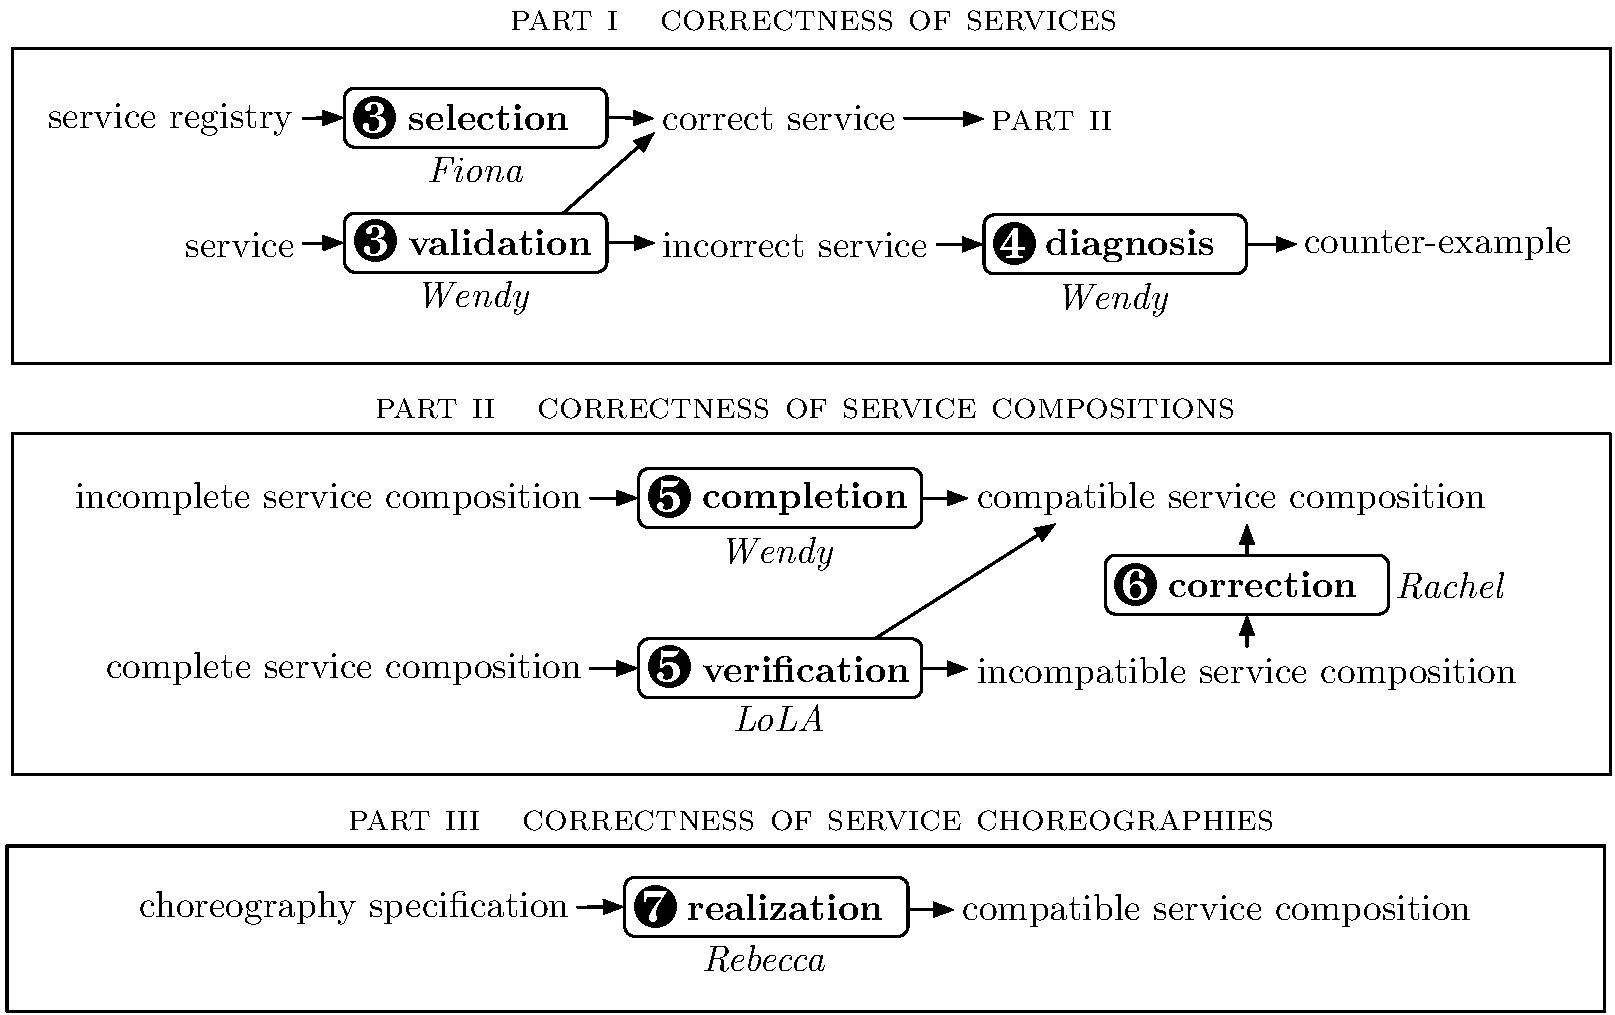
\includegraphics[scale=0.4]{introduction/parts}
\caption{Interrelation of the \textbf{results}, \ding{183} chapters, and \emph{tools}.}\label{fig:parts}
\end{figure}
%%%%%%%%%%%%%%%%%%%%%%%%%%%%%%%%%%%%%%%%%%%%%%%%%%%%%%%%%%%%%%%%%%%%%%%%%%%%%%

The next chapter provides the basic definitions and notions we employ throughout the thesis. It introduces the formal framework we use to model services and service compositions. Furthermore, the correctness criteria introduced informally in this chapter are defined in terms of the formal model. Finally, existing concepts to represent the set of partners of a service are briefly recapitulated.

\medskip

The remainder of the thesis is divided into three parts, each studying a service-oriented system from a different point of view. We present the software tools used and experimental results obtained within the context of the respective chapters.

\begin{niceitemize}
\item \spacedlowsmallcaps{Part I}.\quad The first part is dedicated to correctness criteria which can be expressed and checked with respect to a single service. The refinement of the controllability notion to validate  services is described in \autoref{chap:validation}, together with various application scenarios of this notion, for instance the selection of services from a service registry. \Autoref{chap:diagnosis} focuses on diagnostic information (viz.\ the construction of counterexamples) in case a service is uncontrollable.

\item \spacedlowsmallcaps{Part II}.\quad In the second part, we go one step further and consider the correctness of service compositions. In \autoref{chap:verification}, we show how compatibility of industrial service compositions defined in \bpelchor{} can be verified and how a completion algorithm can support the construction of compatible compositions. \Autoref{chap:correction} shows how correction proposals for incorrect service compositions can be automatically derived.

\item \spacedlowsmallcaps{Part III}.\quad In the last part of the thesis, we study a correctness-by-construction approach for service compositions. Given a choreography specification, we investigate whether this global specification can be realized by several services. \Autoref{chap:realizability} shows how the realizability problem of services can be approached in terms of controllability. This link makes all results of the previous chapters applicable to service choreographies.
\end{niceitemize}

\medskip

\Autoref{chap:conclusion} concludes the thesis and summarizes the contributions and the remaining open problems. Furthermore, it sketches directions for future extensions of the presented results.
